\documentclass[11p]{article}
% Packages
\usepackage{amsmath}
\usepackage{graphicx}
\usepackage{fancyheadings}
\usepackage[swedish]{babel}
\usepackage[
    backend=biber,
    style=authoryear-ibid,
    sorting=ynt
]{biblatex}
\usepackage[utf8]{inputenc}
\usepackage[T1]{fontenc}
%Källor
\addbibresource{references.bib}
\graphicspath{ {./images/} }

% Lite variabler
\def\email{samuel.viglundsson@ga.ntig.se}
\def\foottitle{PMmall}
\def\name{Samuel Viglundsson}

\title{PMmall \\ \small Gymnasiearbete}
\author{\namn}
\date{\today}

\begin{document}


% fixar sidfot
\lfoot{\footnotesize{\name \\ \email}}
\rfoot{\footnotesize{\today}}
\lhead{\sc\footnotesize\foottitle}
\rhead{\nouppercase{\sc\footnotesize\leftmark}}
\pagestyle{fancy}
\renewcommand{\headrulewidth}{0.2pt}
\renewcommand{\footrulewidth}{0.2pt}

% i Sverige har vi normalt inget indrag vid nytt stycke
\setlength{\parindent}{0pt}
% men däremot lite mellanrum
\setlength{\parskip}{10pt}

\maketitle

\section{Bakgrund}
Min frågestälnning är hur gamification(spelifiering) samt spel-baserad inlärning(game-based learning) fungerar i praktiken.


Gamification är att ta delarna som gör spel roliga in i lärande t.ex ha ett narrativ/story för det man gör, poäng system för att göra uppgifter, levlar och bossbattles, direkt feedback av arbete, achievements, tävla mot andra spelare eller dig själv. Jag kommer dels se vad rådande kunskapsläget är gällande gamficaitions effektvietet, dels se hur lärare och sånt känner om gamficifaiton och om det är någonting de använder i lärandet, och sist tänkte jag hålla något experiment där klassen(antaglig vår) får lära sig något nytt och några får lära sig med hjälp av gamfiication och andra inte för att se om det är någon skillnad. Inte ett perfekt experiment då inlärningstiden är så kort men det funkar.

\section{Metod}
Vi kommer att testa grupper av elever, där grupperna är NTI klasser eller gurndskole lasser om vi av någon anledning inte skulle få tillgång till nti klasser. Grupperna delas slumpmässigt in i två delgrupper (a) spelifierade och (b) icke-spelifierade. Grupp (a) kommer att öva 15-20 minuter genom ett gameshow spel på wordwall bestående av 20 frågor, varje fråga har ett ord på islänska(eller annat språk) med fyra alternativ på svenska varav ett av dem är rätt. Eleven uppmuntras, men behöver inte, använda gameshow spelets inbyggda funktioner s.som tidbonusar, eliminera två felaktiga svar, dubbla poäng för rätt svar, osv. Grupp (b) kommer att ges ett papper med de islänska orden och desskorresponderande  översättningar, ingen mera information. Efter 15-20 minuter kommer eleverna att testas genom ett traditionellt skrivtest där översättningnar från svenska till islänska och vice-versa ska anges.

\subsection{Frågor} Originella frågan var initialt hur effektivt spelifiering är för inlärning, en annan naturligt fråga som spelar in i den originella är hur spelifiering påverkar motivering eller frågna vilka former av spelifiering som fungerar bäst(väldigt bred fråga där)

\subsection{Hur hänger frågorna ihop} Motivering bör påverka inlärning och olika former av spelifierings effektivetet är såklart relevant.

\subsection{Urval} Kommer ta skolklasser från NTI, men OM det inte skulle räcka kan jag ta från grundskoleelever. Vi delar på grupperna slumpmässigt. Jag kommer att trakassera lärare/klassföreståndare tills jag får göra experimentet på eleverna.

\subsection{Analys} Jag kommer såklart beräkna saker som medelvärde och felmarginal, kommer även använda regression för att se om vi kan hitta samband mellan spelifiering och resultat. Då resultaten är oparade, vad vi kan anta vara normalfördelade, så kan vi använda oparade T-testet för att testa om vår hypotes att ‘spelifiering ger bättre inlärning’ är sann givet datan.

\section{Referenser}
Då gamification som koncept är ganska nytt finns inte speciellt många studier som pratar om just gamficiations effektivetet som jag har förståt det. Jag ska läsa delar av 'Det Spelifierade klassrummet' av Adam Palmquist för refrenser om vad exakt gamifictaion är och hur man använder det. Jag ska även intervjua en lärare på dragonen som specialiserar sig på gamification: Niclas Lind heter han, Niclas har jättemycket erfarenhet med gamification. Jag ska spela in intervjuvn(givetviss kollade jag så det är okej innan, det är okej) och kan skicka kopia till er sen om ni vill. Jag tror att boken och Niclas kunskap kommer att räcka som källor för de mesta, men kan hända att jag tar upp någonting mer om jag känner det skulle behövas.
\section{Annat som kan vara bra att veta}
Det är lätt att skriva matematik i \LaTeX

\begin{equation}
    F = G \frac{M m}{r^2}
    \label{eq:grav}
\end{equation}

Ekvation (\ref{eq:grav}) känner ni igen...
\clearpage
\subsection{En underrubrik}
    \begin{figure}[!h]
        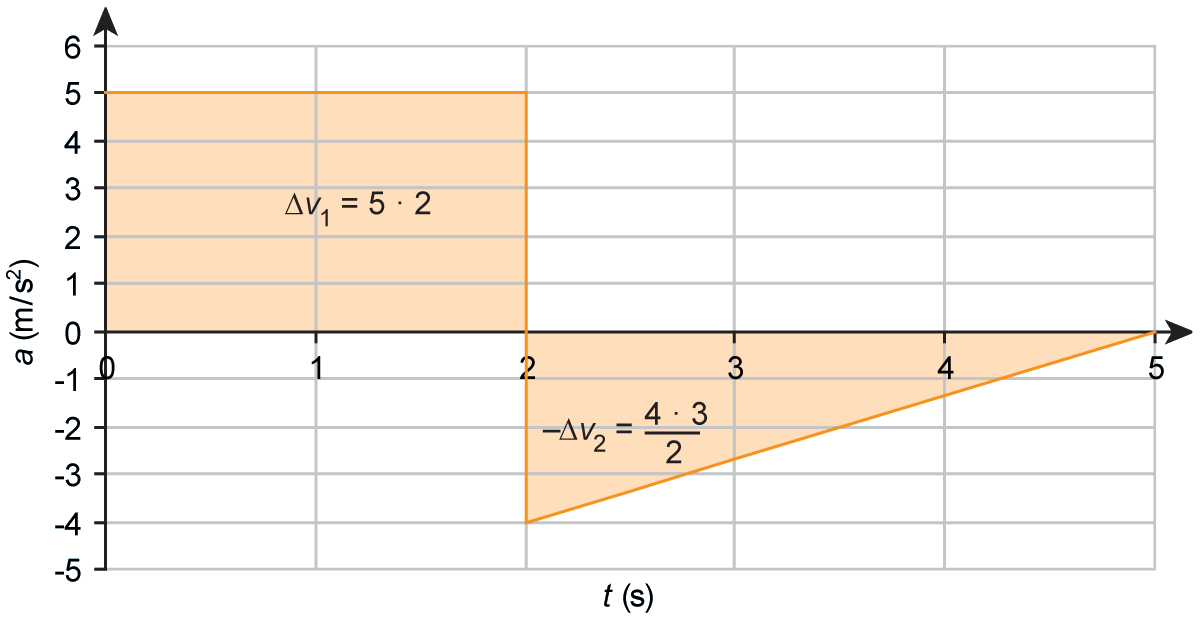
\includegraphics[width=0.8\textwidth]{accelerationTime.png}
        \caption{Acceleration-tid diagram. Källa: \textcite{Fraenkel}}
        \label{fig:acc}
    \end{figure}

Acceleration-tiddiagram (se figur \ref{fig:acc})

\printbibliography

\end{document}
